\documentclass{article}
\usepackage[shortlabels]{enumitem}
\usepackage{amsmath}
\usepackage{amssymb}
\usepackage{stmaryrd}
\usepackage{xcolor}
\usepackage{siunitx}
\usepackage{pgfplots}
\pgfplotsset{compat=1.18}
\usepgfplotslibrary{fillbetween}

\usepackage{xcolor}
\newcommand{\mathcolorbox}[2]{\colorbox{#1}{$\displaystyle #2$}}

\newtheorem{definition}{Definition}

\begin{document}

\begin{definition} \underline{Berechnung des Flacheinhalts A} zwischen $G_f$ und der x-Achse über [a;b] mit $f(x) \geq 0$ f.a. $x \in [a; b]$
\[A = \lim_{n\to \infty} S_n = \lim_{n\to \infty} [f(z_1) + \dotsc + f(z_n)]\cdot \Delta x\]
\center{also}
\[\Delta x \to 0\text{ für }n \to \infty\]

Man nimmt eine Funktion f \underline{integrierbar}, wenn für ale Rechtecksummen $S_n$ gilt 
\[ A = \lim_{n\to \infty}U_n = \lim_{n\to \infty} S_n = \lim_{x\to \infty} O_n \; \; (U_n \leq S_n \leq O_n) \]

\end{definition}

\underline{Bemerkung}

Für stetige Funktionen f gilt: 
\begin{enumerate}[i)]
\item alle $\lim_{n\to \infty} S_n$ existieren,
\item für alle $z_n $ ist dieser Grenzwert gleich,
\item $U_n \leq S_n \leq O_n$

\[ \Rightarrow A = \lim{n\to \infty} S_n = \lim_{n\to \infty} O_n = \lim_{n\to \infty} U_n\]
\end{enumerate}

Beispiel:

\[f(x) = x^2 \;, \; I = [0;2]\]
Bestimmunug des Flächeinhalts zwischen $G_f$ und der x-Achse mit dem Grenzen $ a=0 \; ; \; b = 2$

Man kann zeigen: 
\[1^2+2^2+3^2 + \dots + (n-1)^2 = \frac 16(n-1)\cdot n \cdot (2n-1)\]

die Untersumme $U_n $ mit Stutzstellen und Intervalbreite
\[\Delta x = \frac 2n \quad z_1 = 0 ; z_2 = \frac 2 n ; z_3 = 2\frac 2 n ; z_4 =3\frac 2 n ; z_n = (n-1)\frac 2n\]
\[\Rightarrow U_n = (f(z_1) + \dotsc + f(z_n))\cdot \frac 2 n = (0^2 + (\frac 2n)^2 + (2\frac 2n)^2 + \dotsc + ((n-1)\frac 2n)^2)\cdot \frac 2n\]
\[ U_n = ((\frac 2n)^2+(\frac 2n)^2\cdot 2 + \dotsc + (n-1)^2\cdot (\frac 2n)^2)\cdot \frac 2n\]
\[\rightarrow U_n = (1+2^2 + 3^2 + \dotsc + (n-1)^2 ) \cdot (\frac 2n)^2\cdot \frac 2n\]
\[U_n = \frac 16 (n-1)n(2n-1) \frac 8 {n^3}\]
\[U_n = \frac 43 (n-1) n (2n-1)\frac a{n^3}\]
\[U_n = \frac 43 \frac{(n-a)}n \frac nn \frac {(2n-1)}n\]
\[U_n= \mathcolorbox{red}{\frac 43 (1-\frac1n)(2-\frac1n)}\]

\[A = \lim_{n\to\infty}U_n = \lim_{n\to\infty}\frac 43 (1-\frac 1n)(2-\frac 1n) = \frac 83\approx 2,67\]

Man kann zeigen: für den Flächeinhalt über ü [0;b] gilt: 
\[A = \frac 13 b^3\]

\begin{definition}
\underline{orientierter Flächeinhalt}
Sei f eine auf [a;b] differenzierbare Funktion, dann gilt für den orientierte Flächeinhalt A; den der Graph von f mit der x-Achse über [a;b] einschließt.
\[A = \lim_{n\to\infty} (f(z_1)+\dots+f(z_k))\cdot \Delta x + \lim_{n\to\infty}(f(z_{k+1} + \dots + f(z_n))\cdot \Delta x\]

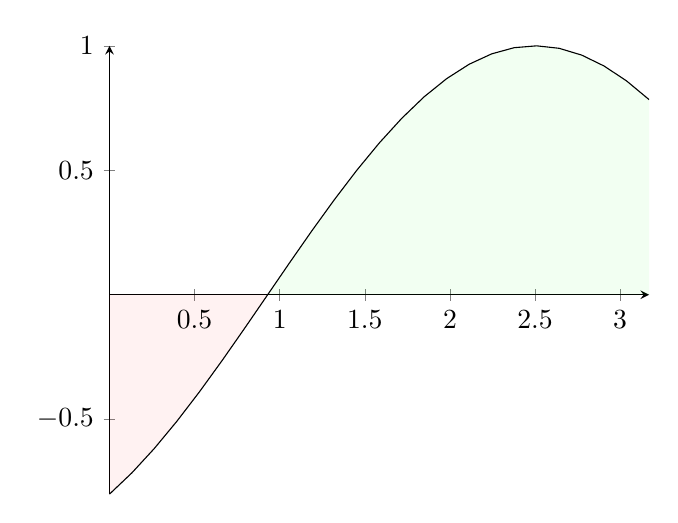
\begin{tikzpicture}
\begin{axis}[
	domain = 0:3.17,
	axis lines = middle,
]
\addplot[name path = f]{-sin(deg(x-180))};
\path[name path=axis] (axis cs:0,0) -- (axis cs:3.17,0);
\addplot [
        thick,
        color=green,
        fill=green, 
        fill opacity=0.05
    ]
    fill between[
        of=f and axis,
        split,
        every segment no 0/.style={
            %fill=none,
            red,
        },
    ];
\end{axis}
\end{tikzpicture}

\[ \textcolor{red}{-A_{unten}} + \textcolor{green}{A_{oben}}\]

\end{definition}

\begin{definition}

Sei f auf I = [a;b] differenzierbar, dann versteht man unter dem \underline{bestimmten Integral von f in den Grenzen vor a bis b}, die \underline{Summe der orientierten Flächeinhalte}, der Teilflächen zwischen der x-Achse der Graphen von f un den Parralleln $x=a; x=b$.

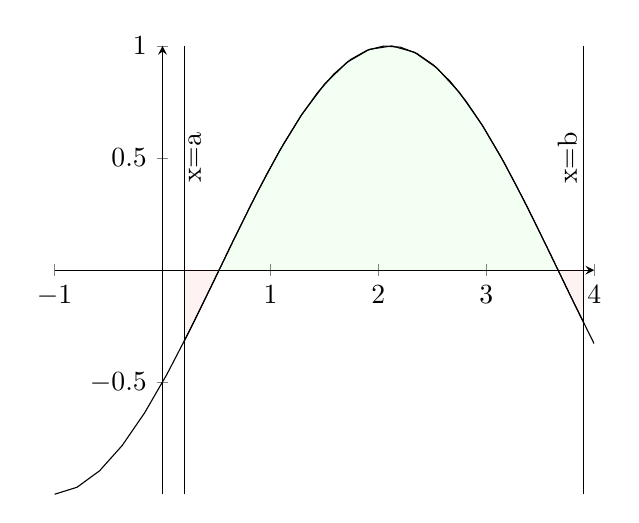
\begin{tikzpicture}
\begin{axis}[
	domain = -1:4,
	axis lines = middle,
]
\addplot[]{sin(deg(x)-30)};
\addplot[name path = f, domain=0.2:3.9]{sin(deg(x)-30)};
\draw [name path = vert-a](0.2,0 |- current axis.south) -- (0.2,0 |- current axis.north);
\node [rotate = 90]at (axis cs: 0.3,0.5) {x=a};
\draw [name path = vert-b](3.9,0 |- current axis.south) -- (3.9,0 |- current axis.north);
\node [rotate = 90]at (axis cs: 3.75,0.5) {x=b};
\path[name path=axis] (axis cs:0.2,0) -- (axis cs:3.9,0);
\addplot [
        thick,
        color=green,
        fill=red, 
        fill opacity=0.05,
    ]
    fill between[
        of=f and axis,
        split,
        every segment no 0/.style={red,},
        every segment no 1/.style={green,},
        every segment no 2/.style={red,},
    ];

\end{axis}
\end{tikzpicture}

\[\int_a ^b f(x) dx = \textcolor{red}{-A_1} + \textcolor{green}{A_2} \textcolor{red}{-A_3}\]
\end{definition}

\[\int_{\text{untere Grenze}}^{\text{obere Grenze}}\text{ Integrand Integrationsvariable}\]

Bemerkung: \underline{Intervaladitivität}
\[\int_a^d f(x) dx = \int_a^b f(x) dx+ \int_b^c f(x) dx + \int_c^d f(x) dx\]

\section{Flächeinhalt als Dreieckflecher}
\[\int_1^4 3x-6 \;dx =\textcolor{red}{-A_1}+\textcolor{green}{A_2} = -\frac 32\]

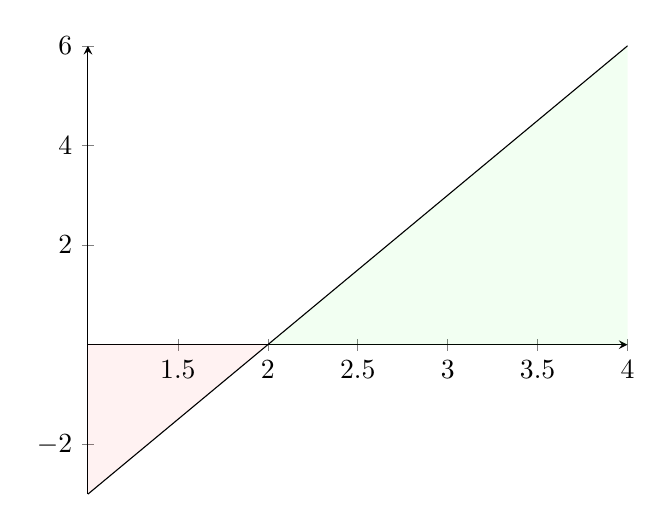
\begin{tikzpicture}
\begin{axis}[
	domain = 0.5:4.5,
	axis lines = middle,
]
\addplot[name path = f, domain = 1:4] {3*x-6};
\path[name path=axis] (axis cs:0,0) -- (axis cs:4,0);
\addplot [
        thick,
        color=green,
        fill=green, 
        fill opacity=0.05,
    ]
    fill between[
        of=f and axis,
        split,
        every segment no 0/.style={
            %fill=none,
            red,
        },
    ];
\end{axis}
\end{tikzpicture}

\begin{definition}Eine differenzierbare Funktion $ F: x \rightarrow F(x)$ heißt \textbf{Stammfunktion} der Funktion $f: \rightarrow f(x); x \in D$, über dem Intervall $ I = [a;b] (I \subseteq D_f)$ falls gilt:
\[F'(x) = f(x) \text{ für alle } x\in I\]

\end{definition}

\begin{definition}
Sind F und G Stammfunktionen von f über dem Intervall I = [a;b], dann gibt es eine Konstante $c \in \mathbb{R}$ 
\[\text{mit } F(x) = G(x) + c \text{ f.a. } x\in I\]
\end{definition}

\begin{definition}(Hauptsatz der Integral- und Differentialrechnung, Formel von Newton-Leibniz)
\\
Sein f auf I = [a;b] differenzierbar und F eine beliebige zu f gehörende Stammfunktion, dann gilt: 
\[ \int_a^bf(x) dx = F(b) - f(a) = [F(x)]_a^b\]

\end{definition}





\end{document}